% Peta jalan TKT + ajakan pilot.
\documentclass[border=4pt]{standalone}
% Gaya bersama gambar deck Demo Day (dipakai semua gambar/*.tex standalone).
\usepackage{amssymb}
\usepackage{fontspec}
\setmainfont{DejaVu Sans Condensed}
\setsansfont{DejaVu Sans Condensed}
\newfontfamily\judulfont{DejaVu Sans}[BoldFont={DejaVu Sans Bold}, Ligatures=TeX]
\usepackage{tikz,pgfplots}
\pgfplotsset{compat=1.18, every axis/.append style={/pgf/number format/assume math mode=true, /pgf/number format/use comma, /pgf/number format/1000 sep={.}}}
\usetikzlibrary{positioning,arrows.meta,calc,shapes.geometric,fit,backgrounds}
\definecolor{gelap}{HTML}{15242B}
\definecolor{teal}{HTML}{285052}
\definecolor{amber}{HTML}{E8A317}
\definecolor{muda}{HTML}{DCE8E8}
\definecolor{abu}{HTML}{8A9499}
\definecolor{teks}{HTML}{1E2B30}
\definecolor{hijau}{HTML}{2F7D5B}
\definecolor{merah}{HTML}{A33A2A}
\color{teks}
\tikzset{
  ubin/.style={fill=muda, rounded corners=5pt, align=center, inner sep=6pt},
  inti/.style={ubin, fill=gelap, text=white},
  panah/.style={-{Stealth[length=3mm]}, line width=1.3pt, draw=amber},
  panahabu/.style={-{Stealth[length=2.5mm]}, line width=1pt, draw=abu},
  judulubin/.style={font=\judulfont\bfseries},
}
% Dibuat otomatis oleh buat_aset.py dari ml/results/energi_harian.json; jangan diedit manual.
\newcommand{\energiTurbin}{270}
\newcommand{\energiQa}{187}
\newcommand{\energiQb}{377}
\newcommand{\hariEnergi}{140}
\newcommand{\raspiWh}{71}
\newcommand{\chipWh}{4,1}
\newcommand{\raspiPersen}{26}
\newcommand{\chipPersen}{1,5}
\newcommand{\raspiPersenA}{19}
\newcommand{\raspiPersenB}{38}
\newcommand{\raspiPersenNum}{26.3}
\newcommand{\chipPersenNum}{1.5}
\newcommand{\hematKwh}{24}
\newcommand{\kaliHemat}{17}
\newcommand{\jRaspi}{182}
\newcommand{\jChip}{10,4}
\newcommand{\periodeEnergi}{2026-03-31--2026-10-20}

\AtBeginDocument{\hyphenpenalty=10000 \exhyphenpenalty=10000}

\begin{document}
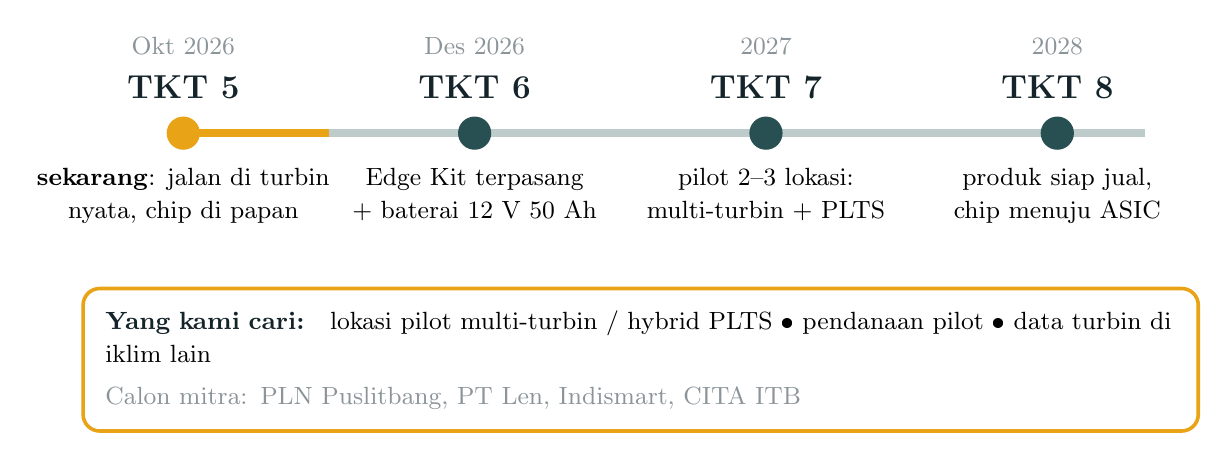
\begin{tikzpicture}[x=3.7cm, font=\fontsize{9.5}{12}\selectfont]
  \draw[line width=3pt, teal!30] (0,0) -- (3.3,0);
  \draw[line width=3pt, amber] (0,0) -- (0.5,0);
  \foreach \x/\t/\k/\b/\c in {0/Okt 2026/TKT 5/{\textbf{sekarang}: jalan di turbin\\nyata, chip di papan}/amber,
                              1/Des 2026/TKT 6/{Edge Kit terpasang\\+ baterai 12 V 50 Ah}/teal,
                              2/2027/TKT 7/{pilot 2--3 lokasi:\\multi-turbin + PLTS}/teal,
                              3/2028/TKT 8/{produk siap jual,\\chip menuju ASIC}/teal}
    {\fill[\c] (\x,0) circle (6pt);
     \node[above=9pt, font=\judulfont\bfseries\fontsize{12}{14}\selectfont, text=gelap] at (\x,0) {\k};
     \node[above=25pt, text=abu] at (\x,0) {\t};
     \node[below=9pt, align=center] at (\x,0) {\b};}
  \node[draw=amber, line width=1.3pt, rounded corners=6pt, text width=13.6cm, align=left, inner sep=8pt, anchor=north west] at (-0.35,-1.95)
    {{\judulfont\bfseries\color{gelap} Yang kami cari:}\quad lokasi pilot multi-turbin / hybrid PLTS \textbullet{} pendanaan pilot \textbullet{} data turbin di iklim lain\\[3pt]
     {\color{abu}Calon mitra: PLN Puslitbang, PT Len, Indismart, CITA ITB}};
\end{tikzpicture}
\end{document}
